\documentclass{beamer}

\usepackage[utf8]{inputenc}
\usepackage{microtype}
\usepackage[T1]{fontenc}
\usepackage{lmodern}
\usepackage[dutch]{babel}
\usepackage{booktabs}
\usepackage{algorithm2e}
\usepackage{siunitx}
\mode<presentation>


\usetheme{Frankfurt}

\author{\hspace{-1 cm}Philippe Tanghe\hspace{1 cm}\and Li Quan}
\title{Traveling Tournament Problem}
\date{30 maart 2011}
\subtitle{Simulated Annealing}
\subject{TTSA}


\AtBeginSection[]{\begin{frame}\frametitle{Inhoudsopgave}\tableofcontents[currentsection]\end{frame}}

\begin{document}
\begin{frame}
\titlepage
\end{frame}

\begin{frame}{Inhoudsopgave}
\tableofcontents%[pausesections]
\end{frame}


\section{Inleiding}
\begin{frame}{Inleiding}
\begin{itemize}
 \item Aris Anagnostopoulos, Laurent Dominique Michel, Pascal Van Hentenryck en Yannis Vergados. \\\emph{A simulated annealing approach to the traveling tournament problem.} (2006)  \pause

\item Pascal Van Hentenryck en Yannis Vergados. \\\emph{A Traveling Tournament Scheduling: A Systematic Evaluation of Simulated Annealing.} (2006)\pause\vspace{1cm}
 
 \item  Traveling Tournament Simulated Annealing Algorithm (TTSA)
\begin{itemize}
 \item SA: goede metaheuristiek voor TTP 
 \item duidelijk en concreet
 \item P.\ Van Hentenryck is een Belg
\end{itemize}
\end{itemize}
\end{frame}



\section{TTSA}

\subsection*{Algoritme}
\begin{frame}{Basisalgoritme SA}

\begin{algorithm}[H]\tiny
find random schedule $S$\;
bestSoFar $\leftarrow$ cost($S$)\;
phase $\leftarrow$ 0\;
\While{phase $\leq$ maxP}
{
 	counter $\leftarrow$ 0\;
 	\While{counter $\leq$ maxC} 
	{
 		select a random move $m$ from neighborhood($S$)\;
 		let $S'$ be the schedule obtained from $S$ with $m$\;
		$\Delta{} \leftarrow$ cost($S'$) - cost($S$)\;
 		\eIf{$\Delta{}<0$ } 
 			{
 			accept $\leftarrow$ true\; 
 			}
 			{
 			accept $\leftarrow$ true with probability $\exp{(-\Delta{}/T)}$\;
 			}

		\If{accept}
			{
 			$S \leftarrow\ S'$\;
 			\eIf{cost(S') $<$ bestSoFar} 
				{
 				counter $\leftarrow$ 0; phase $\leftarrow$ 0\;
 				bestSoFar $\leftarrow$ cost($S'$)\;
				}
				{
 				counter$++$\;
				}
			}
 		
		phase++\;
	$T \leftarrow$ $T\cdot\beta$\;
	}
}
\end{algorithm}

\end{frame}





\subsection*{Eigenschappen TTSA}
\begin{frame}{Eigenschappen TTSA} 
\begin{itemize}
\item<1-> hard en soft constraints
\item<2-> neighborhood van grootte $\mathcal{O}(n^3)$
\item<3-> strategic oscillation
\item<4-> reheats
\end{itemize}
\end{frame}



 \begin{frame}{Hard en soft constraints}
Voorstelling schedule

 \begin{center} \scriptsize
 \begin{tabular}{c | *{10}{r} }
  \textbf{T\textbackslash{}R} & 1 & 2 &3 & 4 & 5 & 6 & 7 & 8 & 9 & 10 \\ \hline
 1 &     6&-2&4&3&-5&-4&-3&5&2&-6 \\
 2 &    5&1&-3&-6&4&3&6&-4&-1&-5\\
 3 &    -4&5&2&-1&6&-2&1&-6&-5&4\\
 4 &    3&6&-1&-5&-2&1&5&2&-6&-3\\
 5&    -2&-3&6&4&1&-6&-4&-1&3&2\\
 6 &  -1&-4&-5&2&-3&5&-2&3&4&1 \\
 \end{tabular}
 \end{center}

\begin{itemize}
\scriptsize{
 \item T teams; R rounds
\item + home; - away }
\end{itemize}


\begin{itemize}
 \item constraints
\begin{itemize}
 \item hard: double round-robin
 \item soft: atmost \& norepeat
\end{itemize}
\end{itemize}



\end{frame}


\subsection*{Local search}
\begin{frame}{Local search}

\begin{itemize} \item initieel random schedule \pause

\begin{itemize}
 \item eenvoudige recursieve backtrack search \pause   %inefficient, alternatieven? grafiek of tabel
\end{itemize}

\item kies $S'$ in neighborhood van $S$ \pause
\begin{itemize}
\item SwapHomes($S,T_i,T_j$) 
\item SwapRounds($S,r_k,r_l$)
\item SwapTeams($S,T_i,T_j$)
\item PartialSwapRounds($S,T_i,r_k,r_l$)
\item PartialSwapTeams($S,T_i,T_j,r_k$) 
\end{itemize} \pause


\item aanvaard of verwerp $S'$
\end{itemize}


\end{frame}

\begin{frame}{Voorbeeld PartialSwapTeams}
PartialSwapTeams($S,T_2,T_4,r_9$)

  \begin{center} \footnotesize
 \begin{tabular}{c | *{10}{r} }
  \textbf{T\textbackslash{}R} & 1 & 2 &3 & 4 & 5 & 6 & 7 & 8 & 9 & 10 \\ \hline
 1 &     6&-2&4&3&-5&-4&-3&5&2&-6 \\
 2 &    5&1&-3&-6&4&3&6&-4&\alert{-1}&-5\\
 3 &    -4&5&2&-1&6&-2&1&-6&-5&4\\
 4 &    3&6&-1&-5&-2&1&5&2&\alert{-6}&-3\\
 5&    -2&-3&6&4&1&-6&-4&-1&3&2\\
 6 &  -1&-4&-5&2&-3&5&-2&3&4&1 \\
 \end{tabular}
 \end{center}

\end{frame}

\begin{frame}{Voorbeeld PartialSwapTeams}
PartialSwapTeams($S,T_2,T_4,r_9$)

  \begin{center} \footnotesize
 \begin{tabular}{c | *{10}{r} }
  \textbf{T\textbackslash{}R} & 1 & 2 &3 & 4 & 5 & 6 & 7 & 8 & 9 & 10 \\ \hline
 1 &     6&-2&\alert{2}&3&-5&-4&-3&5&\alert{4}&-6 \\
 2 &    5&1&\alert{-1}&\alert{-5}&4&3&6&-4&\alert{-6}&\alert{-3}\\
 3 &    -4&5&\alert{4}&-1&6&-2&1&-6&-5&\alert{2}\\
 4 &    3&6&\alert{-3}&\alert{-6}&-2&1&5&2&\alert{-1}&\alert{-5}\\
 5&    -2&-3&6&\alert{2}&1&-6&-4&-1&3&\alert{4}\\
 6 &  -1&-4&-5&\alert{4}&-3&5&-2&3&\alert{2}&1 \\
 \end{tabular}
 \end{center}

\end{frame}

\subsection*{Objectieffunctie}
\begin{frame}{Objectieffunctie}

Objectieffunctie
 \begin{equation*}
  C(S)=%
  \begin{cases}
    cost(S) &\textrm{als $S$ feasible is,} \\
    \sqrt{cost(S)^2 + [w\cdot{}f(nbv(S))]^2} &\textrm{anders}.
  \end{cases}
\end{equation*} \pause

\begin{itemize}[<+->]
 \item $cost(S)$: afstandskost
\item $nbv(S)$: \# violations (soft) constraints
 \item $w$: gewichtsfactor
\item $f(v)=1+(\sqrt{v}\ln{v})/\lambda$
\begin{itemize}
\item sublineair, eerste violation kostelijker ($f(1) = 1$)
\item \footnotesize{($\lambda{}=2$ voor kleine $n$; $\lambda{}=1$ voor grote $n$)}
\end{itemize}
\end{itemize}
\end{frame}

%   \item feasible, infeasible ($\delta=\theta=1.04$)



\subsection*{Uitbreidingen basisalgoritme}
\begin{frame}{Uitbreidingen}

\begin{itemize}
 \item<1-4> strategic oscillation
\scriptsize{
\begin{equation*}
  C(S)=%
  \begin{cases}
    cost(S) &\textrm{als $S$ feasible is,} \\
    \sqrt{cost(S)^2 + [\alert{w}\cdot{}f(nbv(S))]^2} &\textrm{anders}.
  \end{cases}
\end{equation*} } \vspace{-0.4cm}
\begin{itemize}
 \item<2-4> gewichtsfactor $w$ vari\"eren
 \item<2-4> feasible $w \leftarrow w/\theta$; infeasible $w \leftarrow w\cdot\delta$
  
\end{itemize}


 \item<3-4> reheating

\begin{itemize}
 \item<4> lokale minima op lage temperaturen
 \item<4> eenvoudig reheating schema
\end{itemize}
\end{itemize}



 %(2 maal beste temperatuur)
\end{frame}


\section{Implementatie}
\begin{frame}{Implementatie}
\textsc{Matlab} 
\begin{itemize}
 \item[+] snelle implementatie % algoritme + modificaties
 \item[+] matrix- en vectoroperaties 
 \item[+] snel testen
 \item[--] performantie (?)
\end{itemize}
\end{frame}

\section{Experimenten}


\begin{frame}{Experimenten}
\begin{itemize}
 \item random schedule generatie
 \item parameters

\end{itemize}

\end{frame}
\subsection*{Random schedule}

\begin{frame}{Random schedule}
 eenvoudig recursieve backtracking? 
\begin{figure}[H]
 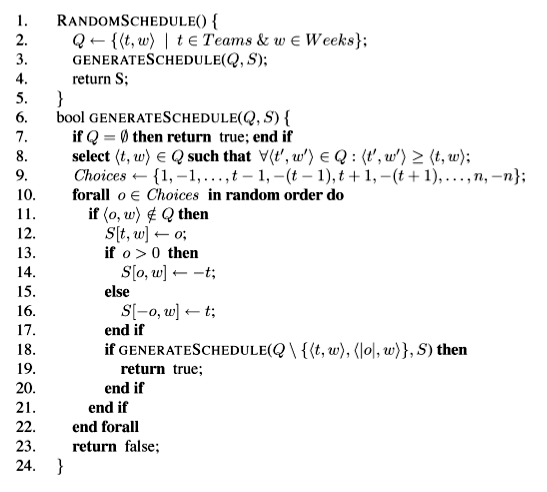
\includegraphics[width=0.75\textwidth]{randomscheduleALG}
\end{figure}
\end{frame}

\begin{frame}{Random schedule}
kleine fout in algoritme
\begin{figure}[H]
 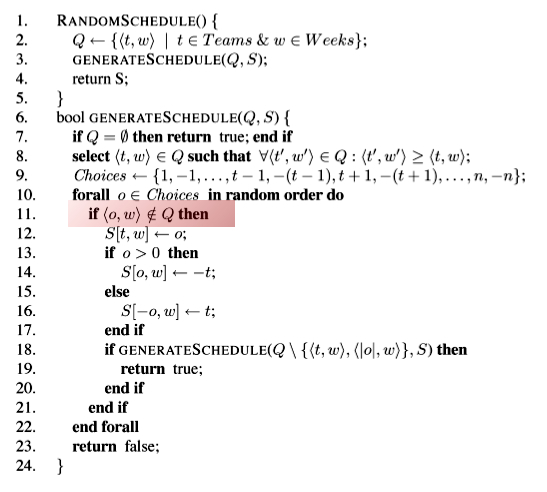
\includegraphics[width=0.75\textwidth]{randomscheduleALG_phixr}
\end{figure}
\end{frame}

\begin{frame}{Random schedule}

\begin{columns}[T]
\begin{column}{0.5\textwidth}
  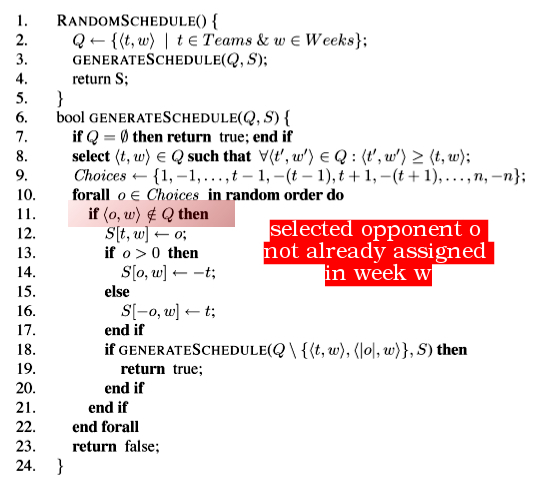
\includegraphics[width=\textwidth]{randomscheduleALG_phixr2}
\end{column}

\begin{column}{0.5\textwidth}
\begin{exampleblock}{Triviaal tegenvoorbeeld $(n=2)$}
 \scriptsize{\begin{itemize}
  \item $Q = \{(1,1);(1,2);(2,1);(2,2)\}$
  \item $(t,w) = (1,1)$
  \item $Choices = \{2,-2\}$
  \item $o = 2 $
  \item $(o,w) = (2,1) \in Q$ 
 \end{itemize}}

\end{exampleblock}\pause
\alert{maar $o$ is beschikbaar}
\end{column}

\end{columns}
\end{frame}

\begin{frame}{Random schedule}
 
\begin{columns}[T]
\begin{column}{0.5\textwidth}
  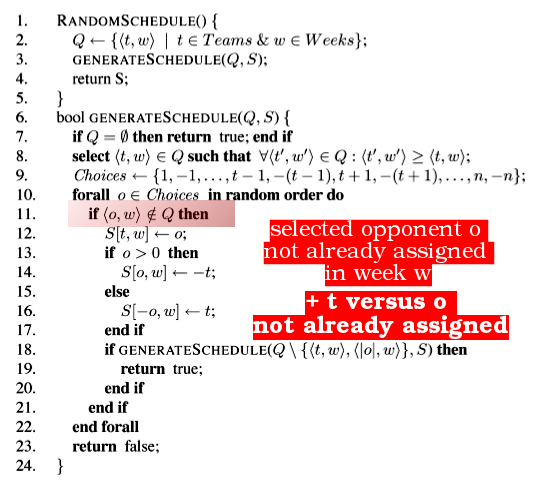
\includegraphics[width=\textwidth]{randomscheduleALG_phixr3}
\end{column}

\begin{column}{0.5\textwidth}
\begin{exampleblock}{Triviaal tegenvoorbeeld $(n=2)$}
 \scriptsize{\begin{itemize}
  \item $Q = \{(1,1);(1,2);(2,1);(2,2)\}$
  \item $(t,w) = (1,1)$
  \item $Choices = \{2,-2\}$
  \item $o = 2 $
  \item $(o,w) = (2,1) \in Q$ 
 \end{itemize}}

\end{exampleblock}

\alert{anders kan team $t$ meerdere keren zelfde wedstrijd tegen $o$ spelen}
\end{column}

\end{columns}

\end{frame}


\begin{frame}{Random schedule}

\begin{columns}[c]
 \begin{column}{0.5\textwidth}
  
scaleerbaarheid:
\begin{itemize}
 \item goed voor NL4--8
 \item ok voor NL10--12
 \item traag voor NL14--16 
\end{itemize}
 \end{column}

 \begin{column}{0.5\textwidth}
  
bottleneck:
\begin{itemize}
 \item shuffle-algoritme \\\tiny{(\texttt{randperm} $\mathcal{O}(n\log{n})$ vs $\mathcal{O}(n)$)} \normalsize
 \item \alert{\#backtracks}
\end{itemize}

 \end{column}

\end{columns}



\pause

\begin{table}[H]
 \centering 
% \begin{center}
\footnotesize
\begin{tabular}{c S S S S }\toprule
$n$ & {min (s)} & {avg (s)} & {max (s)} & {std (s)}  \\\midrule
 4   & 0.004	& 0.006	& 0.009	& 0.002 \\
 6   & 0.011&	0.017&	0.044&	0.010\\
 8  &  0.020	&1.889	&18.558&	5.857  \\
 10  & 0.031	&14.271	&112.291&	35.549\\
 12 &0.055	&8.795	&51.114&	16.583 \\
 14 & 0.089	&96.782	&612.953&	195.414\\
 16  &  1.088&286.021	&923.226	&360.467 \\ 
 \bottomrule
 \end{tabular}
\caption{Tijd nodig om een random schedule te maken via een recursief backtrack algoritme ($N=10$). \label{tab:random}}
\end{table}
\end{frame}

% \plainframe{

% 
% }

\subsection*{Parameters TTSA}
\begin{frame}{Parameters}

parameters \alert{empirisch} bepalen

\begin{itemize}
\item TTSA
\begin{itemize}
 \item traag $\Rightarrow$ \alert{weinig experimenten}
\end{itemize}

\item TTSA (Fast Cooling)
\begin{itemize}
\item beperkte tijd $\Rightarrow$ meer experimenten
\item goede resultaten
\end{itemize}
\end{itemize}

\tiny{
\begin{tabular}{l c c c c c c c c} \toprule
& $T_0$ & $\beta$ & $maxC$ & $maxP$ & $maxR$ & $\delta$ & $\theta$ & $w_0$ \\\midrule
TTSA &  400--700 & 0.9999 & 4000--10000 & 7100 & 10--50 & 1.04 & 1.04 & 4000--60000 \\ 
TTSA(FC) &  400--600 & 0.99 & 100--500 & 100--500 & 1--5 & 1.04 & 1.04 & 4000--10000 \\\bottomrule

\end{tabular}}

\end{frame}


\plainframe{
%figuur TTSA NL6 vs TTSA(FC) 
\begin{figure}[hbpt]
\centering
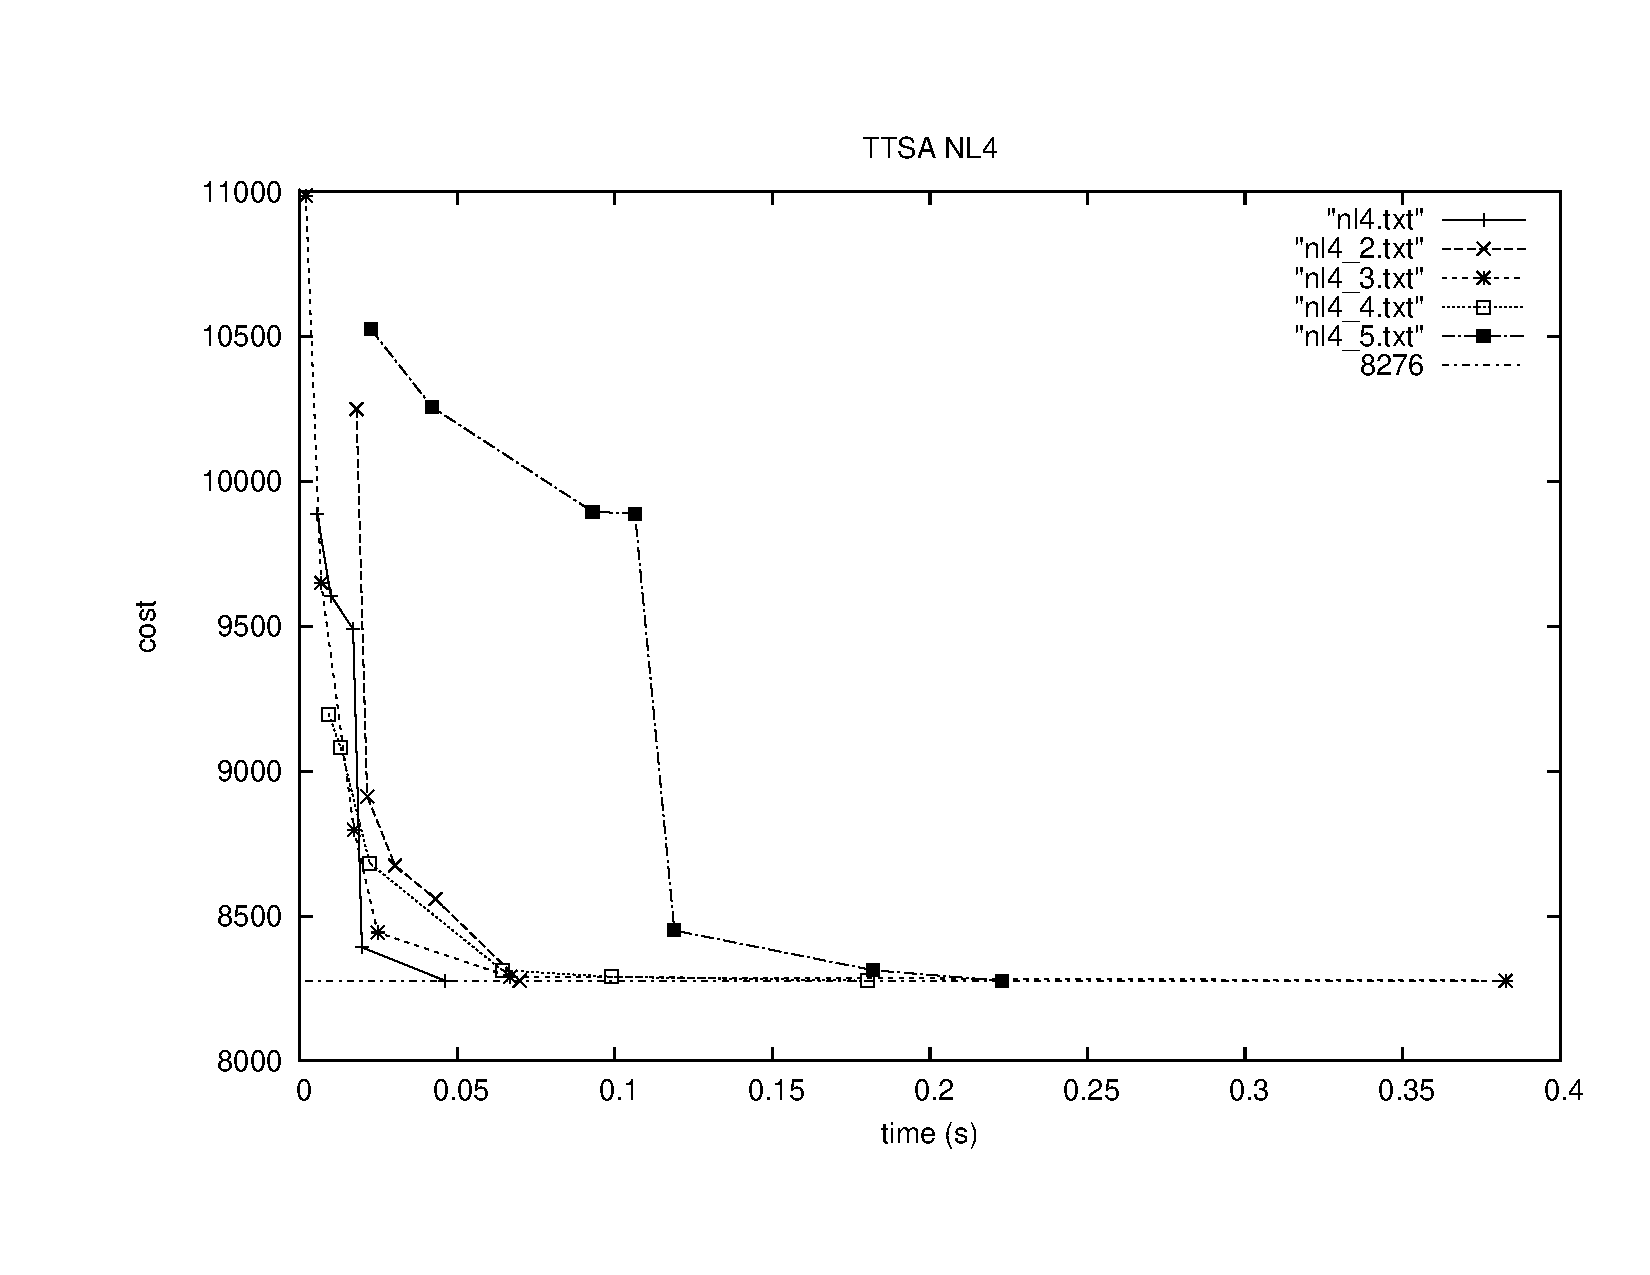
\includegraphics[width=0.95\textwidth,keepaspectratio=true]{../verslag/img/ttsaNL4}
 \caption{TTSA NL4.}
 \label{fig:nl4}
 \end{figure}
}


\plainframe{
%figuur TTSA NL6 vs TTSA(FC) 
\begin{figure}[hbpt]
\centering
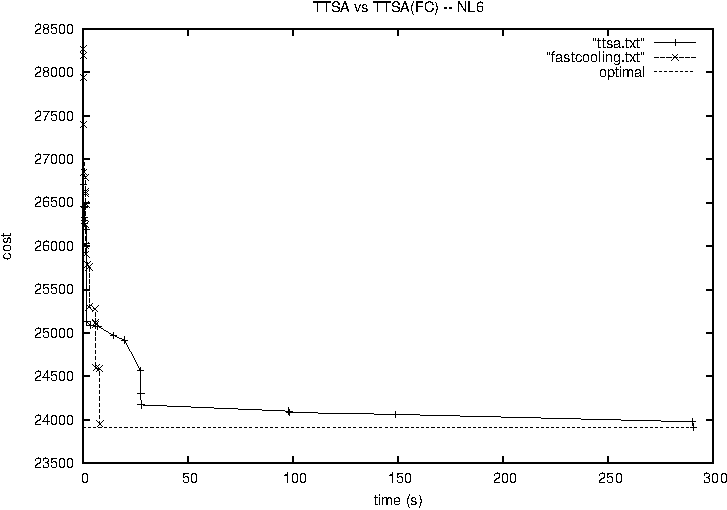
\includegraphics[width=0.95\textwidth,keepaspectratio=true]{../verslag/img/nl6_ttsaVSttsaFC}
 \caption{TTSA vs TTSA(FC) NL6.}
 \label{fig:nl6}
 \end{figure}
}

\plainframe{
\begin{figure}[hbpt]
\centering
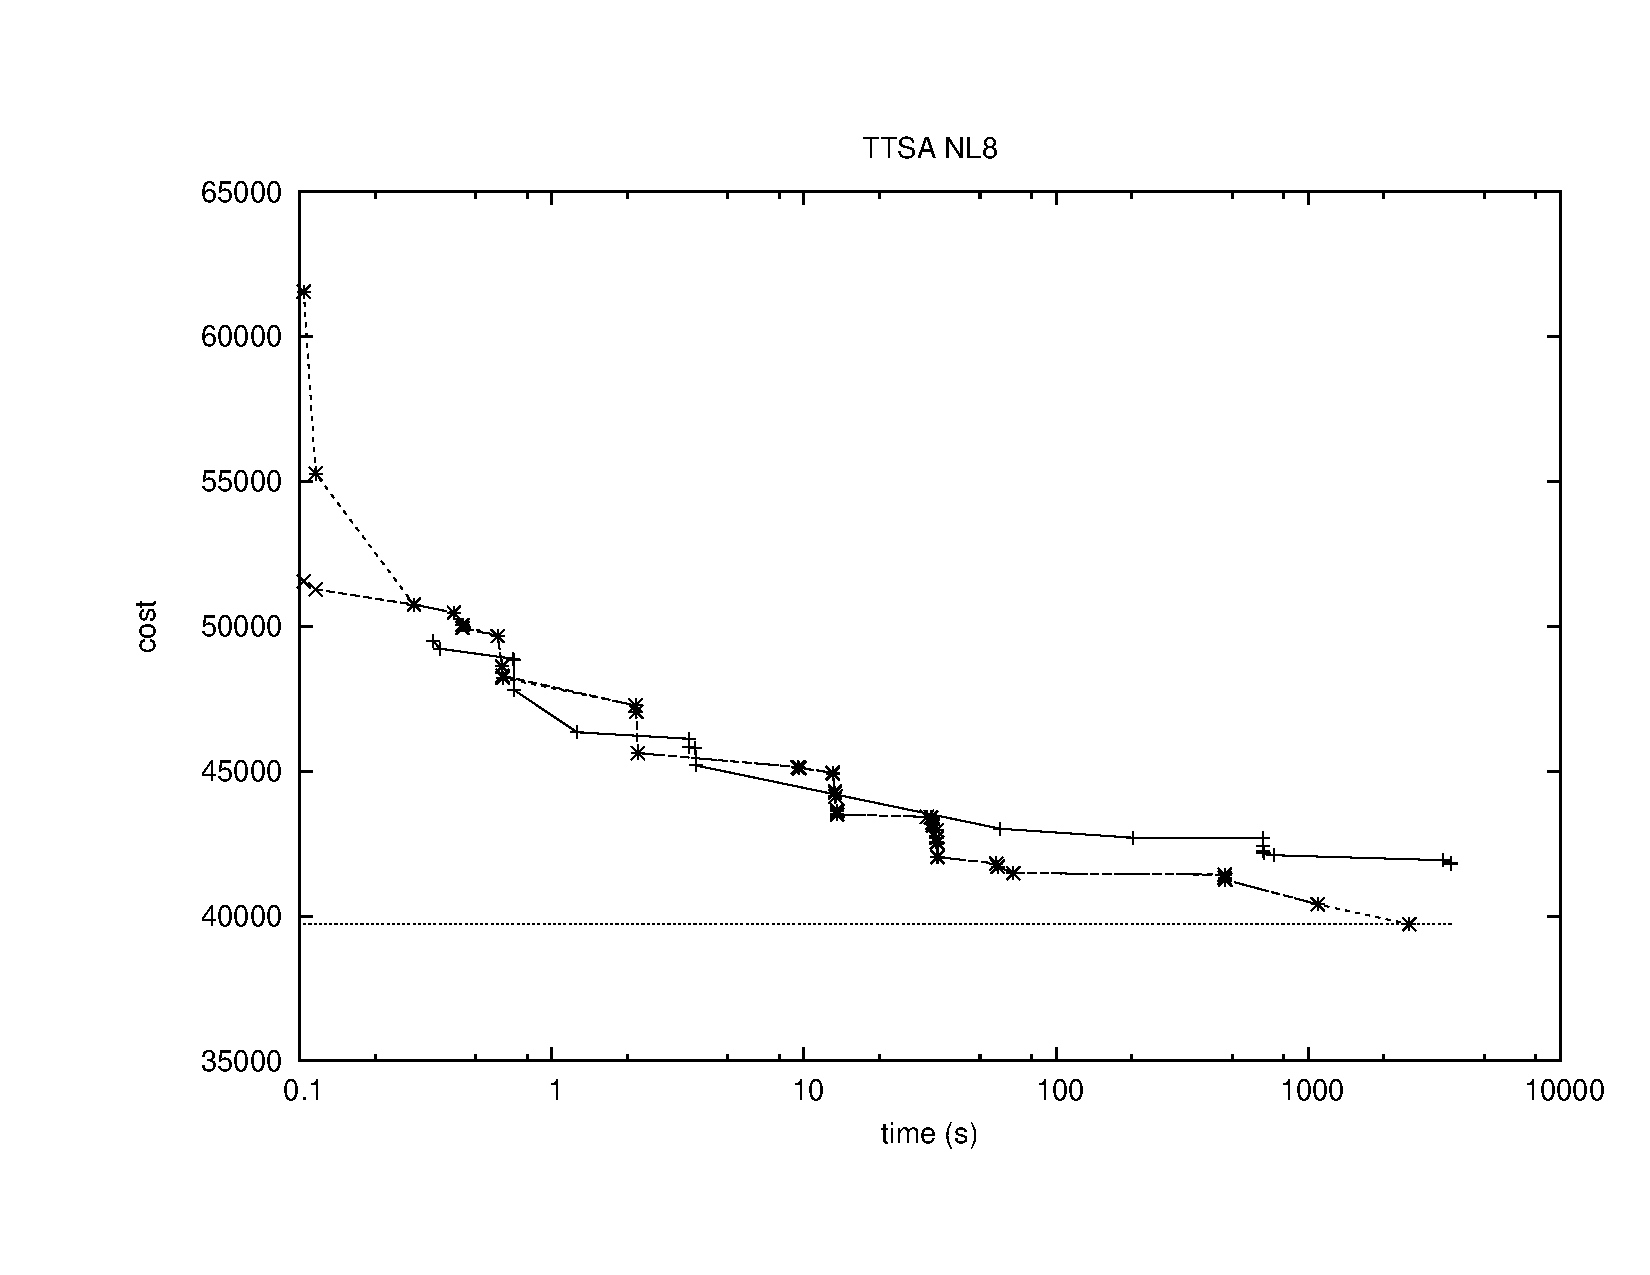
\includegraphics[width=0.95\textwidth,keepaspectratio=true]{../verslag/img/ttsaNL8}
 \caption{TTSA NL8 (logaritmische tijdsas).}
 \label{fig:nl8}
 \end{figure}
}

\plainframe{
\begin{figure}[hbpt]
\centering
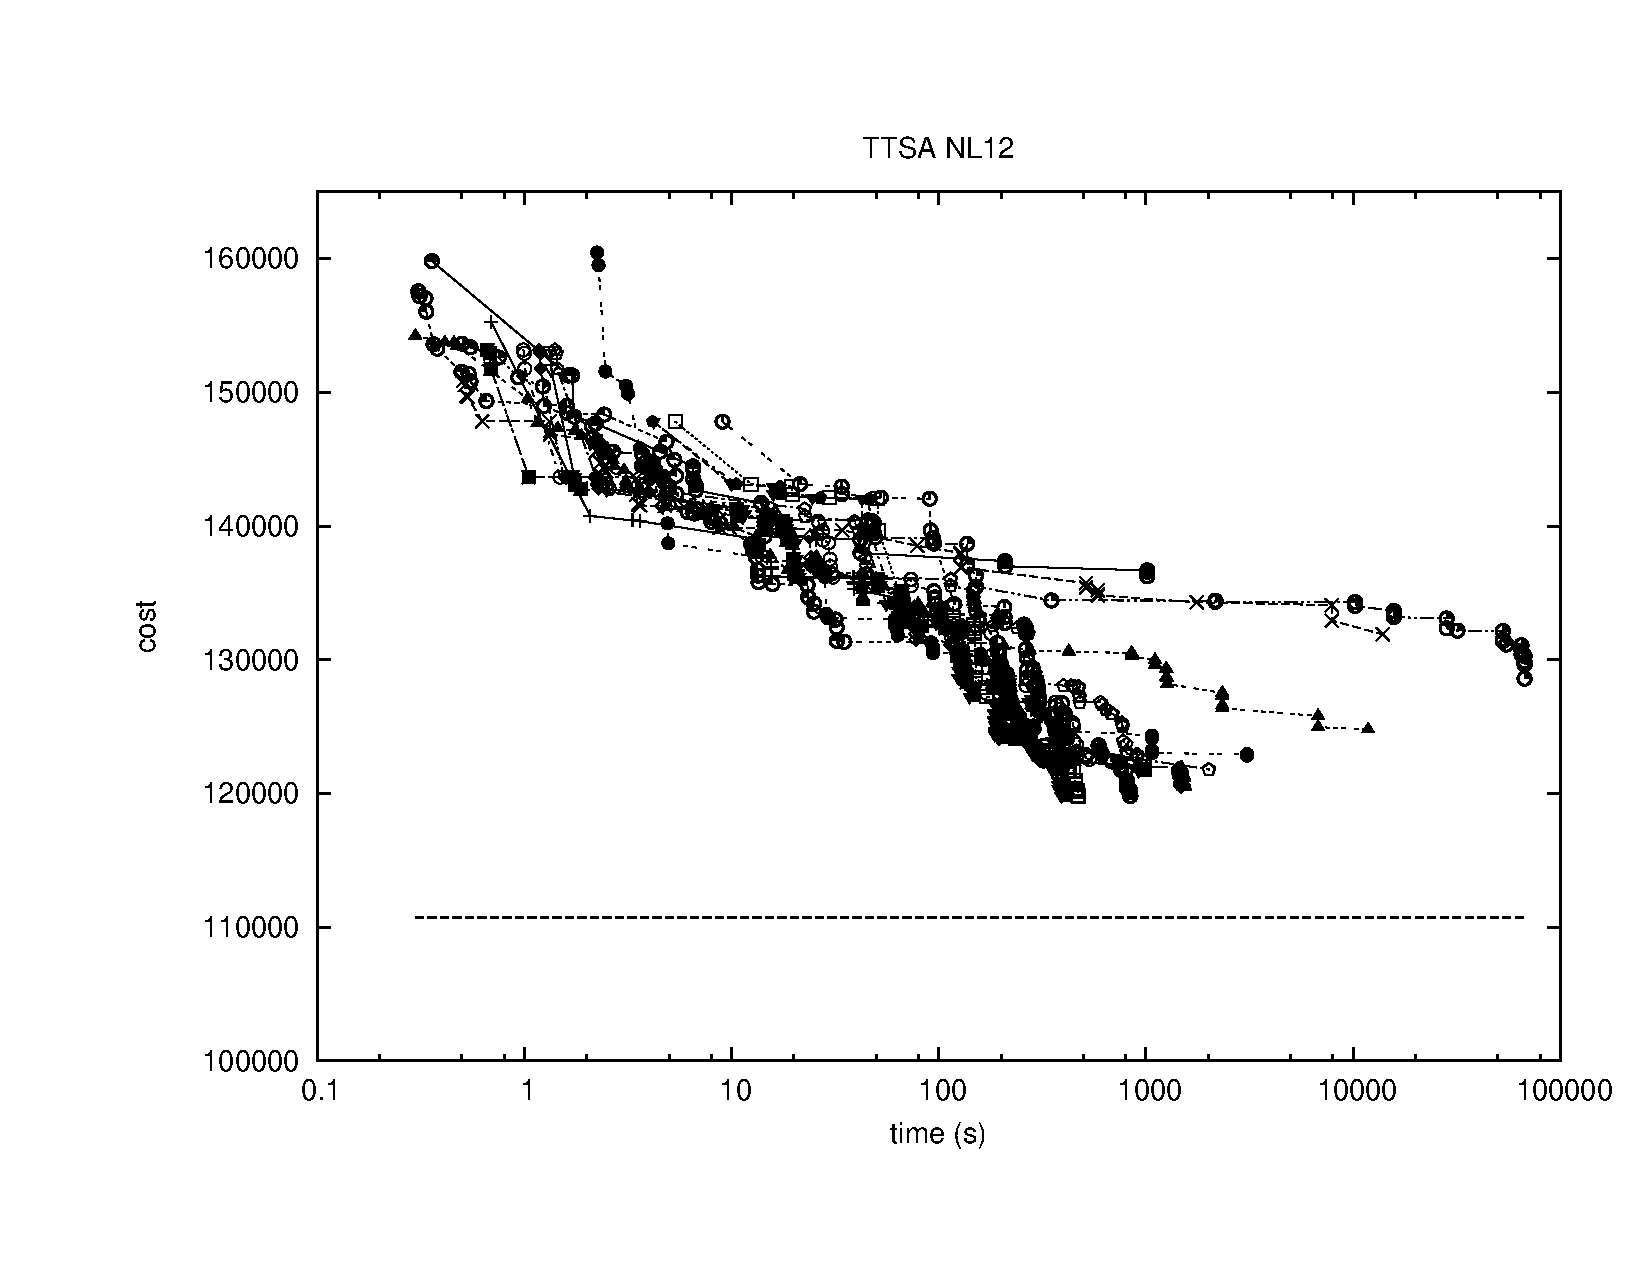
\includegraphics[width=0.95\textwidth,keepaspectratio=true]{../verslag/img/ttsaNL12}
 \caption{TTSA(FC) NL12 (logaritmische tijdsas).}
 \label{fig:nl12}
 \end{figure}
}

\plainframe{
\begin{figure}[hbpt]
\centering
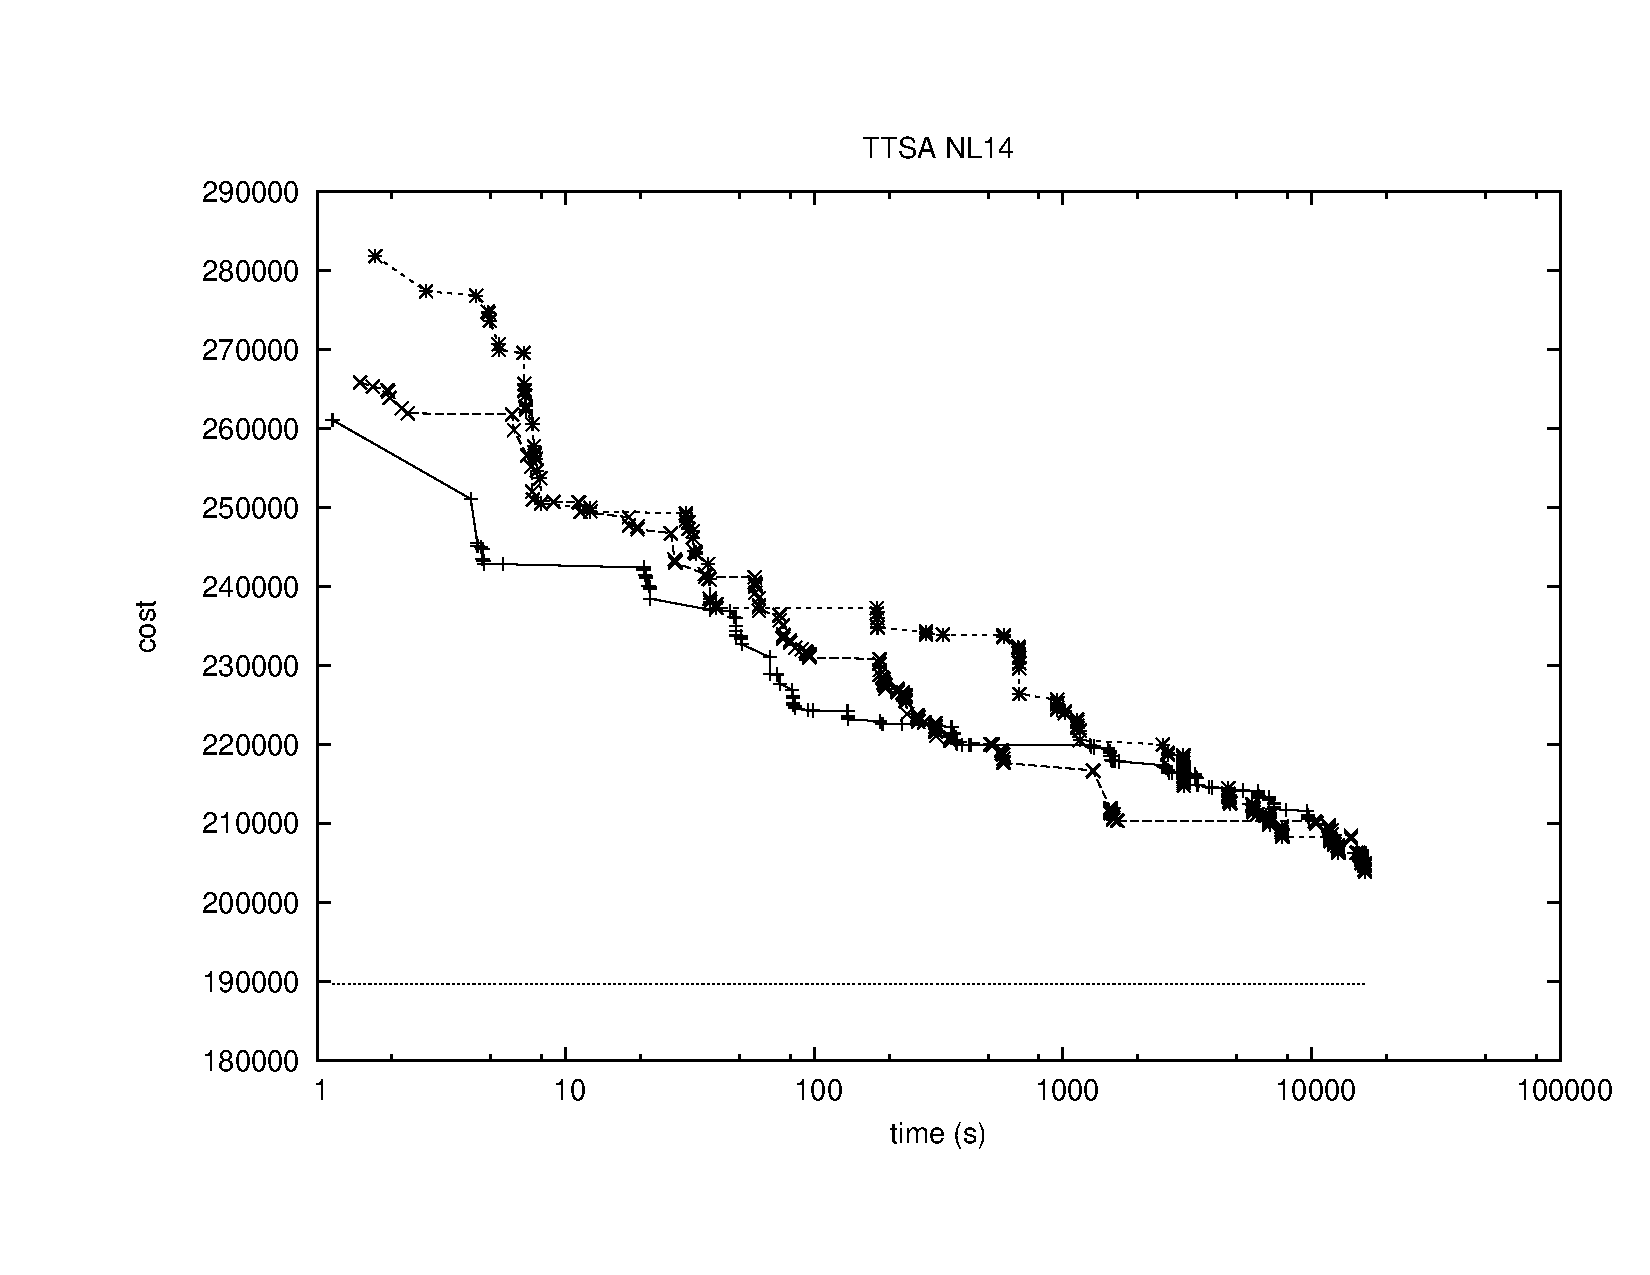
\includegraphics[width=0.95\textwidth,keepaspectratio=true]{../verslag/img/ttsaNL14}
 \caption{TTSA(FC) NL14 (logaritmische tijdsas).}
 \label{fig:nl14}
 \end{figure}
}


\plainframe{
\begin{figure}[hbpt]
\centering
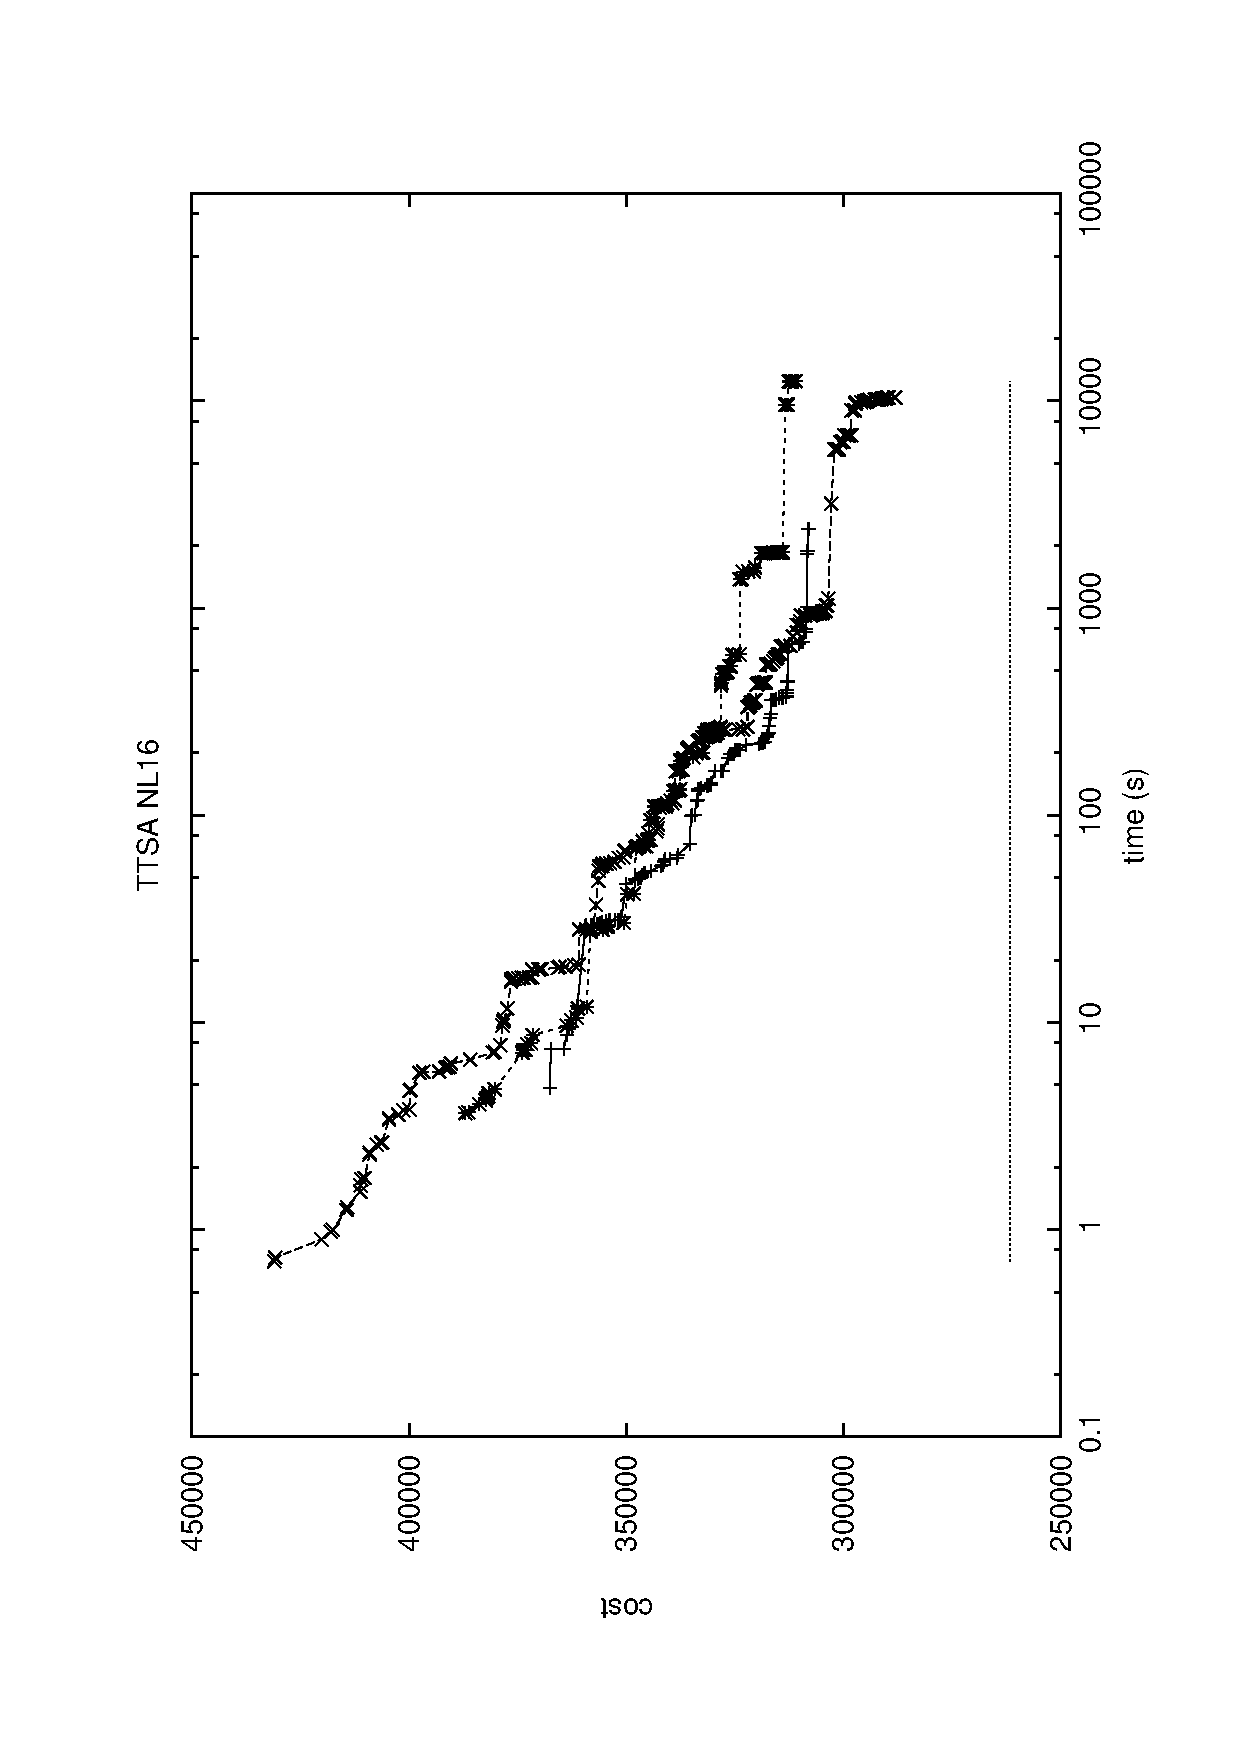
\includegraphics[width=0.95\textwidth,keepaspectratio=true]{../verslag/img/ttsaNL16}
 \caption{TTSA(FC) NL16 (logaritmische tijdsas).}
 \label{fig:nl16}
 \end{figure}
}




\section{Mogelijke verbeteringen}
\begin{frame}{Mogelijke verbeteringen}
\begin{itemize}[<+->]
  \item beter algoritme initieel schedule 
\begin{itemize} 
\item randomized hill-climbing: Dinitz en Stinson. \\\emph{A Hill-climbing Algorithm for the Construction of One-Factorizations and Room Squares}. (1987)
\item constraint programming? 
\end{itemize}
  \item parameters TTSA
\begin{itemize}
  \item random restart
  \item neighborhood
  \item \ldots
\end{itemize}


\end{itemize}
 \end{frame}

\begin{frame}{Mogelijke verbeteringen (2)}
 \begin{itemize}[<+->]
  \item uitbreidingen naar niet NL-instanties. \\Van Hentenryck en Vergados. \\\emph{A Traveling Tournament Scheduling: A Systematic Evaluation of Simulated Annealing.} (2006)
  \item hybride algoritme, e.g.~population-based SA. \\Van Hentenryck en Vergados. \\\emph{Population-based simulated annealing for traveling tournaments}. (2007)
  \item \ldots
\end{itemize}
\end{frame}



\section{Conclusie}
\begin{frame}{Conclusie}
\begin{itemize}[<+->]
 \item matige resultaten TTSA
 \item goede resultaten TTSA(FC)
 \item empirisch bepalen parameters

\end{itemize}


\end{frame}

\begin{frame}{Conclusie}


 \begin{tabular}{c r r r r r r r }\toprule
 $n$ && cost  & && best (2002) &  TTSA (2003) &best (2010)  \\\midrule
 4   && \emph{8276}  & && 8276            &	8276 &8276  \\
 6   && \emph{23916} & && 	23916     &  23916 &23916 \\
 8   && \emph{39721} & &&	  39721   &  39721 &39721  \\
 10  &&  63667     && & 	61608	& 59583 &59436 \\
 12  &&  \emph{118499}     && &	118955	 &112800 &110729 \\
 14  &&   \emph{203979}    && & 205894		&190368 &188728 \\
 16  && 288089   && &       281660          &267194 &261687 \\
 \bottomrule
 
 \end{tabular}


\end{frame}



% 
% \begin{frame}[plain]
% \begin{center}
% \Huge Vragen?
% \end{center}
% \end{frame} 



% De implementatie van het algoritme TTSA zoals beschreven in~\cite{paper} is in \textsc{Matlab} gedaan. De keuze hiervoor was dat \textsc{Matlab} toelaat om heel vlug volledige programma's te schrijven en de bewerkingen voor de matrices ook heel eenvoudig te gebruiken zijn.
% 
% Het nadeel van een ge\"{\i}nterpreteerde taal ten op zichte van een gecompileerde is uiteraard de performantie; vectoroperaties en de optimisaties van de JIT accelerator voor for-loops zouden deze kloof echter aanzienlijk moeten verkleinen~\cite{matlab}.
% 
% Het recursieve backtrack algoritme om een random schedule te genereren werd ietwat gewijzigd: in de paper stond een fout in het algoritme waardoor soms niet-feasible schedules werden geproduceerd of sommige feasible schedules verworpen. De paper vermeldt ook dat aan dit algoritme weinig aandacht besteed werd en feasible schedules redelijk effici\"ent werden geproduceerd met hun algoritme, hoewel het heel wat verbeterd kan worden~\cite{paper}. In~\cite{paper2} gebruiken ze een beter scaleerbaar algoritme.
% 
% In onze experimenten met ons eigen recursieve backtracking algoritme in \textsc{Matlab} bleek het algoritme perfect te werken voor NL4--10, degelijk voor NL12, en heel slecht voor NL14--16. Uit nader onderzoek blijkt dit te komen door het aantal backtracks; voorlopig wordt echter gewoon het algoritme in deze vorm gebruikt. 





\end{document}

